\documentclass[10pt,twocolumn,a4paper]{ctexart}
\usepackage[margin=1.7cm,columnsep=0.65cm]{geometry}
\usepackage{amsmath,amssymb,bm}
\usepackage{booktabs}
\usepackage{graphicx}
\usepackage{microtype}
\usepackage{natbib}
\usepackage{xcolor}
\usepackage{hyperref}
\usepackage{enumitem}
\usepackage{fancyhdr}

\graphicspath{{../../artifacts/figures/}}
\setlength{\parindent}{2em}
\setlist{nosep,leftmargin=*}
\hypersetup{colorlinks=true,linkcolor=blue!55!black,
  citecolor=green!45!black,urlcolor=blue!65!black}
\pagestyle{fancy}
\fancyhf{}
\fancyhead[L]{Online RL Interview Guide}
\fancyhead[R]{ShaneLiu04}
\fancyfoot[C]{\thepage}

\providecommand{\PPOBest}{--}
\providecommand{\PPOFinal}{--}
\providecommand{\PPOSeeds}{--}
\providecommand{\OffBaseBest}{--}
\providecommand{\OffBaseFinal}{--}
\providecommand{\OffBaseSeeds}{--}
\providecommand{\OffUTDBest}{--}
\providecommand{\OffUTDFinal}{--}
\providecommand{\OffUTDSeeds}{--}
\InputIfFileExists{../results_macros.tex}{}{}

\title{\vspace{-1.2em}\textbf{Online Reinforcement Learning 工程与研究面试指南：\\
从 Bellman Control 到 PPO、Double-Q 与高 UTD}}
\author{ShaneLiu04\\
\small\url{https://github.com/ShaneLiu04}}
\date{}

\begin{document}
\maketitle
\thispagestyle{fancy}

\begin{abstract}
本文构建面向算法工程、机器人学习与强化学习研究岗位的 online RL 知识体系。内容从
MDP、Bellman equation 和 tabular Q-learning 出发，推导 policy gradient、baseline、
GAE、PPO clipped objective、actor-critic、target network、clipped double-Q、critic
ensemble 与 UTD，并以 Meta-World hammer 稀疏奖励实验连接理论、PyTorch 实现、远端
训练、统计评测和系统部署。本文不把面试准备等同于背诵公式，而要求能够解释 estimator
的 bias--variance、识别 bootstrap error、设计有证据力的 ablation，并在 simulator
吞吐、GPU utilization、replay storage 与安全约束之间做工程权衡。
\end{abstract}

\textbf{关键词：}求职面试；Online RL；PPO；Actor-Critic；Q-Learning；
Sample Efficiency；Robot Learning

\section{一张地图理解 Online RL}
强化学习的输入不是固定 label，而是 agent 通过 policy 改变后续数据分布。MDP 记为
$\mathcal M=(\mathcal S,\mathcal A,P,r,\gamma,\rho_0)$。策略目标为
\[
J(\pi)=\mathbb E_{\tau\sim\pi}\left[
\sum_{t=0}^{T}\gamma^t r(s_t,a_t)\right].
\]
面试时可以用四个维度定位算法：
\begin{enumerate}
  \item \textbf{value-based 或 policy-based：}优化 $Q$ 的 greedy policy，还是直接
  对 $\pi_\theta$ 求梯度；
  \item \textbf{on-policy 或 off-policy：}数据是否必须来自当前 policy；
  \item \textbf{model-free 或 model-based：}是否学习或使用 dynamics；
  \item \textbf{Monte Carlo 或 bootstrapping：}target 来自完整 return 还是 learned
  value。
\end{enumerate}
Q-learning 是 off-policy、value-based、model-free、bootstrapped；PPO 是
on-policy、policy-based，并用 critic bootstrap；本作业 actor-critic 是 off-policy、
policy-based，同时学习 ensemble Q-functions。

\section{Bellman Equation 与 Q-Learning}
\subsection{从固定策略到最优控制}
固定策略的 action value 满足
\[
Q^\pi(s,a)=\mathbb E[r+\gamma Q^\pi(s',a')].
\]
最优 Bellman operator 为
\[
(\mathcal T^\star Q)(s,a)=
\mathbb E_{s'}[r+\gamma\max_{a'}Q(s',a')].
\]
$\gamma<1$ 时它在 sup norm 下是 contraction，因此 tabular iteration 收敛到唯一固定点
$Q^\star$\citep{watkins1992qlearning,sutton2018rl}。stochastic approximation 更新只
需采样 transition，不需要知道 $P$。

\subsection{为什么 Q-Learning 是 Off-Policy}
behavior policy 可以用 $\epsilon$-greedy 收集数据，target 却使用
$\max_{a'}Q(s',a')$，对应 greedy target policy。选择 action 的 policy 与学习的 policy
不同，因此是 off-policy。SARSA 使用实际采样的 $a'$，是 on-policy。

\subsection{终止状态的实现}
terminal transition 的 target 应为 $y=r$，不能读取 reset 后新 episode 的 value：
\[
y=r+\gamma(1-d)\max_{a'}Q(s',a').
\]
漏掉 done mask 会把两个 episode 拼接，产生系统性 target bias。这是最常见的 RL
implementation interview bug。

\subsection{Reward Design 不是附属工作}
\begin{figure}[t]
\centering
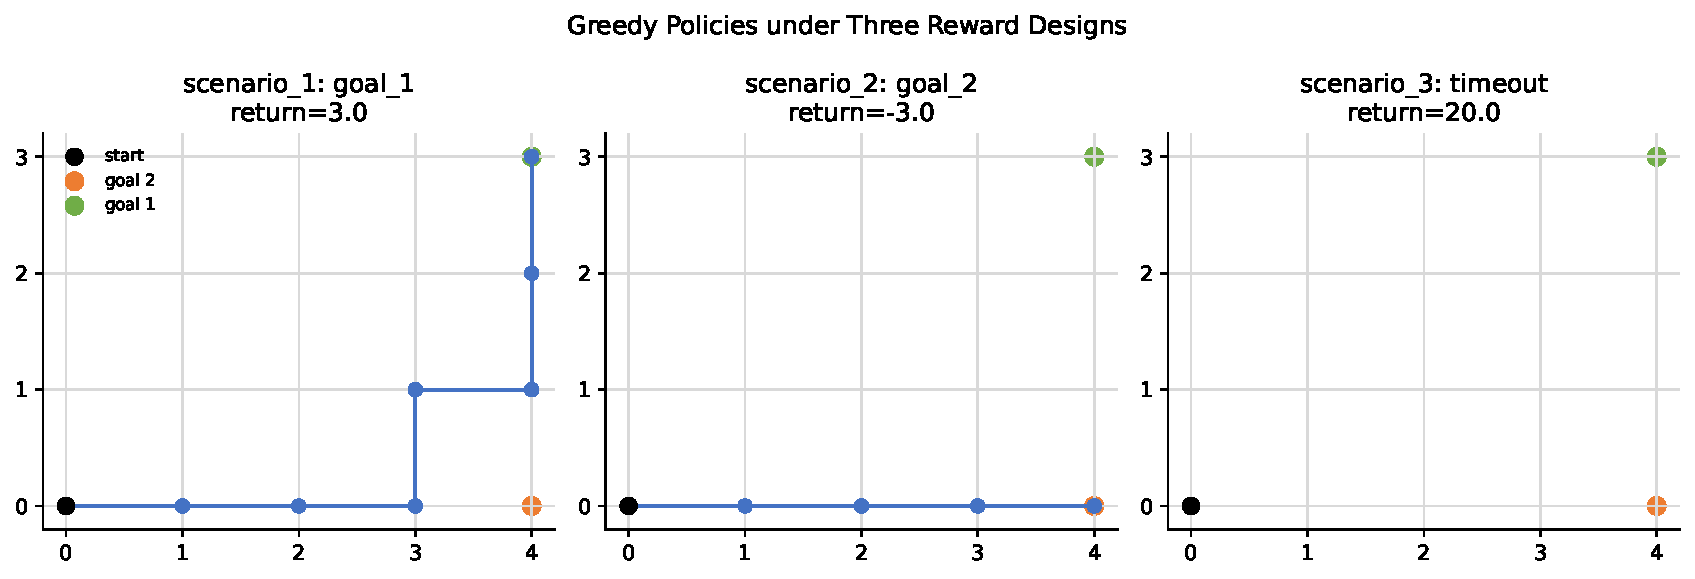
\includegraphics[width=\columnwidth]{gridworld_trajectories}
\caption{相同 dynamics、不同 reward 产生完全不同的最优行为。}
\end{figure}
正 step reward 会鼓励 agent 延迟终止；过大的 negative step cost 会偏好近端低价值
goal。agent “钻漏洞”通常不是 optimizer 错误，而是 proxy objective 与真实意图不一致。
面试回答 reward hacking 时应区分 specification、optimization 与 generalization 三类
failure。

\section{Policy Gradient：从 Log-Derivative 到 Baseline}
trajectory probability 为
$p_\theta(\tau)=\rho_0(s_0)\prod_t
\pi_\theta(a_t|s_t)P(s_{t+1}|s_t,a_t)$。环境 dynamics 不依赖 $\theta$，因此
\[
\nabla_\theta J=
\mathbb E_\tau\left[\sum_t
\nabla_\theta\log\pi_\theta(a_t|s_t)G_t\right].
\]
只使用 reward-to-go 是 causality 的结果：过去 reward 不受当前 action 影响。加入
只依赖 state 的 baseline $b(s_t)$ 不改变期望，因为
$\mathbb E_{a\sim\pi}[\nabla\log\pi(a|s)b(s)]=0$。当
$b=V^\pi$ 时，权重成为 advantage。REINFORCE 无 bootstrap、近似无偏但方差高
\citep{williams1992reinforce}；actor-critic 用 learned value 降低方差，引入
approximation bias。

\section{GAE 的 Bias--Variance 推导}
GAE 是不同 horizon advantage estimators 的指数加权：
\[
\hat A_t^{\rm GAE(\gamma,\lambda)}
=\sum_{l=0}^{\infty}(\gamma\lambda)^l\delta_{t+l},
\quad
\delta_t=r_t+\gamma V(s_{t+1})-V(s_t).
\]
其递推形式只需逆序扫描：
\[
\hat A_t=\delta_t+\gamma\lambda(1-d_t)\hat A_{t+1}.
\]
$\lambda=0$ 为 one-step TD；$\lambda=1$ 在 episode 完整时接近 Monte Carlo return
减 baseline。$\gamma$ 定义 task objective，$\lambda$ 调节 estimator；二者数值同时
出现，但概念不同。

\begin{figure}[t]
\centering
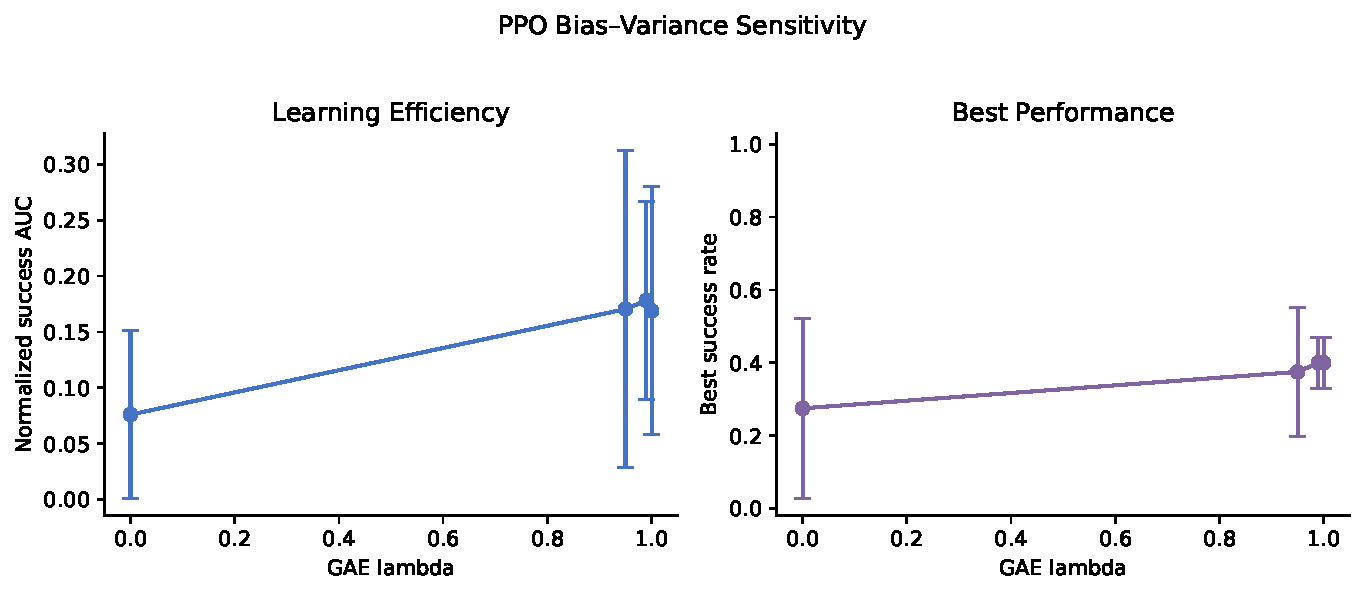
\includegraphics[width=\columnwidth]{gae_lambda_ablation}
\caption{短 budget 下 $\lambda$ 对 learning AUC 与 best success 的影响。}
\end{figure}

\textbf{高频追问：为什么 advantage 要 normalize？}在 minibatch 内标准化不改变样本的
相对顺序，能缓和 reward scale 对 learning rate 的影响；但它改变 gradient scale，
且小 batch 的统计量可能噪声很大。应记录 raw advantage mean/std 以诊断 critic。

\section{PPO：Clip 能保证什么}
\subsection{Importance Ratio}
数据来自 $\pi_{\rm old}$，新策略 objective 用 ratio 修正：
\[
\rho_t=\frac{\pi_\theta(a_t|s_t)}
{\pi_{\rm old}(a_t|s_t)}
=\exp(\log\pi_\theta-\log\pi_{\rm old}).
\]
连续多维 action 的 log-prob 必须对 action dimensions 求和，再计算 ratio。

\subsection{Clipped Surrogate}
\[
L^{\rm clip}=
\mathbb E\left[\min(\rho_tA_t,
\operatorname{clip}(\rho_t,1-\epsilon,1+\epsilon)A_t)\right].
\]
对正 advantage，ratio 过大时收益被截断；对负 advantage，ratio 过小时惩罚被截断。
必须先乘 advantage 再取 minimum，不能简单 clip loss。PPO clip 只约束 sampled actions
上的 surrogate improvement，不是严格 KL bound；因此仍需监控 approximate KL、
clip fraction、entropy 与 value loss。

\subsection{为什么能对同一 Rollout 做多 Epoch}
第一轮后数据已 off-policy，但小 update、clip 和有限 epochs 把 distribution shift 控制在
可接受范围。epochs 太少浪费数据，太多会 overfit advantage noise。TRPO 用显式 KL
constraint 与 conjugate gradient，PPO 牺牲理论约束换取 first-order optimizer 的工程
简洁\citep{schulman2015trpo,schulman2017ppo}。

\section{Off-Policy Actor-Critic}
\subsection{Replay 的价值与代价}
replay buffer 打破 temporal correlation 并提高 transition reuse，显著改善 sample
efficiency。代价是数据来自旧 policies，critic target 和 actor objective 可能在
out-of-distribution actions 上外推。continuous control 中通常通过 target network、
double-Q、policy smoothing 和 entropy/BC regularization 稳定学习。

\subsection{为什么需要 Target Network}
若 target $r+\gamma Q_\phi(s',a')$ 与 prediction $Q_\phi(s,a)$ 同时快速变化，优化目标
成为 moving target。Polyak average
$\bar\phi\leftarrow(1-\tau)\bar\phi+\tau\phi$ 生成慢变量。
$\tau$ 太大失去稳定效果，太小则 target lag 严重。

\subsection{Overestimation 与 Double-Q}
带噪估计满足
$\mathbb E[\max_a\hat Q(s,a)]\ge\max_a\mathbb E[\hat Q(s,a)]$。TD3 用两个 critics
取 minimum，降低 positive bias\citep{fujimoto2018td3}。minimum 可能产生
underestimation；REDQ 从 ensemble 随机抽两个取 min，再更新所有 critics，在 bias、
variance 与计算间折中\citep{chen2021redq}。

\subsection{Actor Gradient}
reparameterized action 可写为
$a_\theta=\tanh(\mu_\theta(s)+\sigma\epsilon)$。actor objective
\[
L_\pi=-\mathbb E_s\left[\frac1N\sum_iQ_{\phi_i}(s,a_\theta)\right]
\]
通过 $Q$ 对 action 的梯度更新 actor。critic parameters 不由 actor optimizer step，
但实现时可临时冻结 critic 以节省 gradient storage。

\section{UTD：样本效率不等于计算效率}
UTD 表示每个 environment transition 对应多少 gradient updates。增大 UTD：
\begin{itemize}
  \item 优点：在真实机器人或 simulator interaction 昂贵时，提高 data reuse；
  \item 风险：对有限 replay support 过拟合，反复传播错误 target；
  \item 成本：GPU FLOPs 与 wall time 增加，即使 environment frames 减少；
  \item 配套：larger ensemble、target network、regularization 与 fresh data ratio。
\end{itemize}

\begin{figure}[t]
\centering
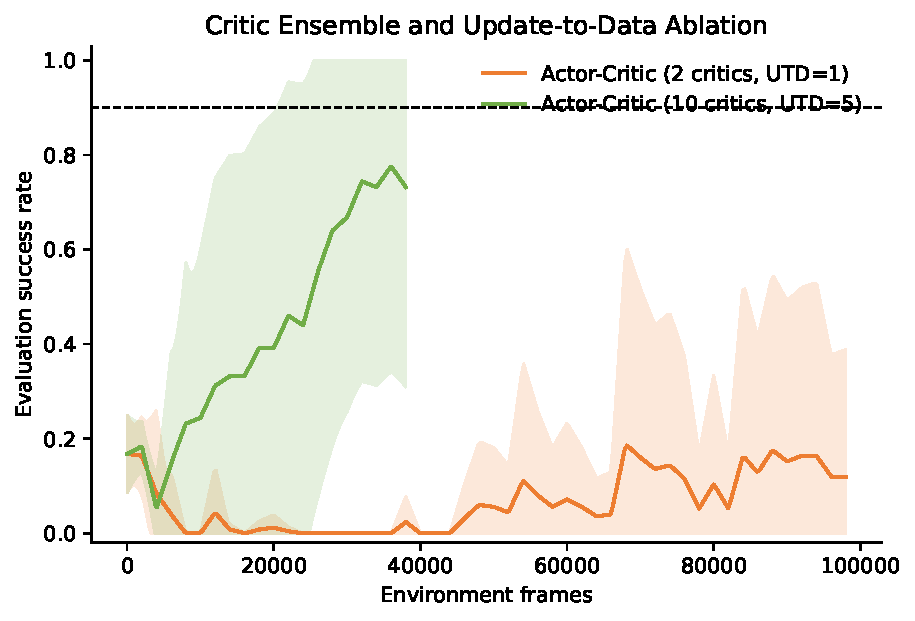
\includegraphics[width=\columnwidth]{off_policy_utd_ablation}
\caption{UTD 与 critic ensemble 对 sample efficiency 的联合影响。}
\end{figure}

\textbf{面试陷阱：}“UTD=5 比 UTD=1 快”必须说明 metric。它可能用更少 environment
frames 达标，却需要更多 gradient steps 或更长 wall time。报告中至少分开
sample efficiency、compute efficiency 与 asymptotic performance。

\begin{figure}[t]
\centering
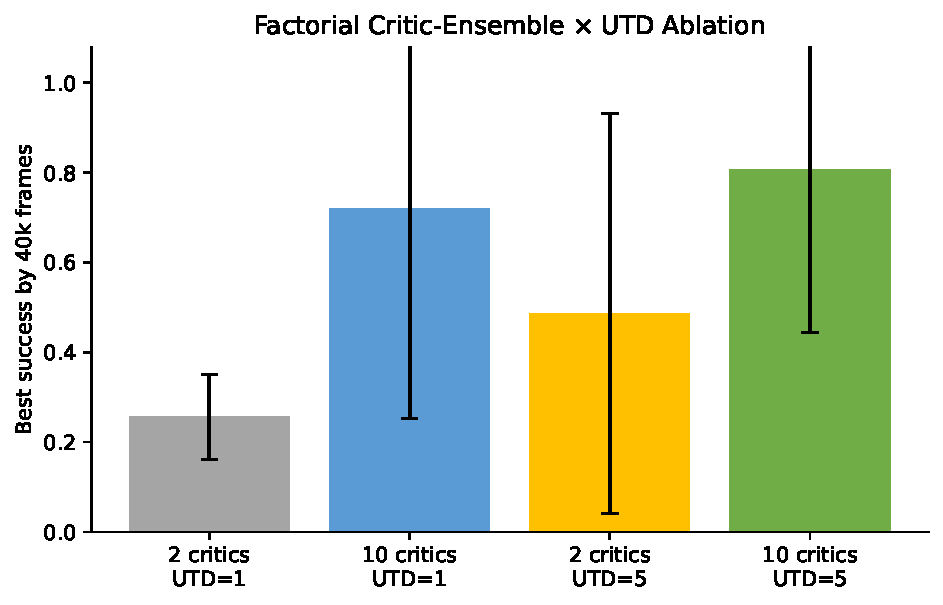
\includegraphics[width=\columnwidth]{critic_utd_factorial}
\caption{$2\times2$ factorial ablation 分离 critic count 与 UTD。}
\end{figure}

若实验同时把 critics 从 2 改为 10、UTD 从 1 改为 5，就无法判断改进来自哪一项。
factorial design 补齐两个交叉配置，是研究面试中“如何修复 confounded ablation”的直接
例子。

\section{Demonstrations 如何跨越 Sparse Reward}
随机 policy 在 hammer task 几乎看不到 success，policy gradient 的 reward-weighted
signal 接近零。BC 把 policy 放到 expert occupancy 附近；off-policy agent 还把
demonstrations 放入 replay，使成功 transition 持续被采样。DDPGfD 与 demonstration
augmented RL 采用类似思路\citep{vecerik2017ddpgfd,nair2018demo}。

但 BC prior 可能限制 improvement。常见策略是：(1) pretrain 后纯 RL；(2) RL 中以较低
频率 interleave BC；(3) advantage-weighted BC；(4) KL to reference policy。regularizer
应随 online evidence 增加逐渐减弱，否则 agent 难以超越 suboptimal expert。

\begin{figure}[t]
\centering
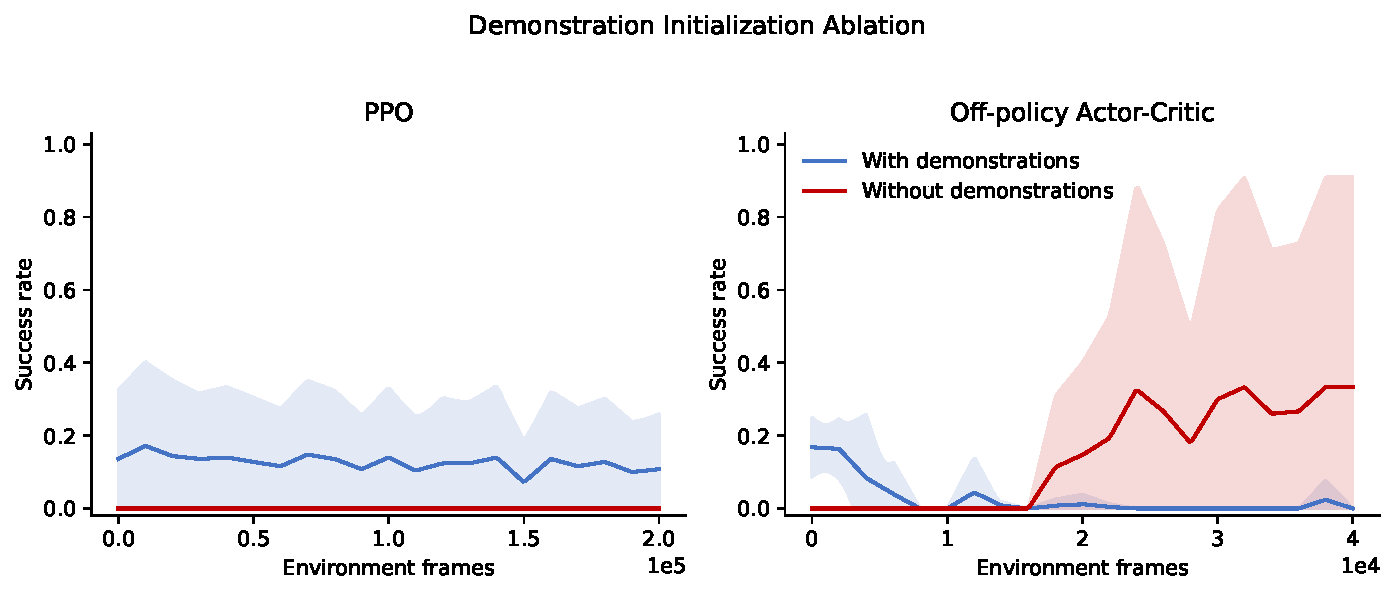
\includegraphics[width=\columnwidth]{demonstration_ablation}
\caption{移除 demonstrations 后的 exploration 对照。}
\end{figure}

高质量 ablation 还需同步移除 PPO 对随机 reference policy 的 KL，否则“no BC”条件仍受
一个无意义先验约束。off-policy 条件则同时设置 pretrain steps 和 interleaved BC
frequency 为零。

\section{实验设计：如何让 RL 结论可信}
\subsection{独立统计单元}
seed 而不是 timestep 是算法稳定性的主要独立重复。evaluation episode 用于估计同一
checkpoint 的 success variance，但不能替代训练 seed。应报告 mean、SD、median、
best/final、seed count 和 evaluation episode count
\citep{henderson2018deep,islam2017reproducibility}。

\subsection{Best 与 Final}
\begin{figure}[t]
\centering
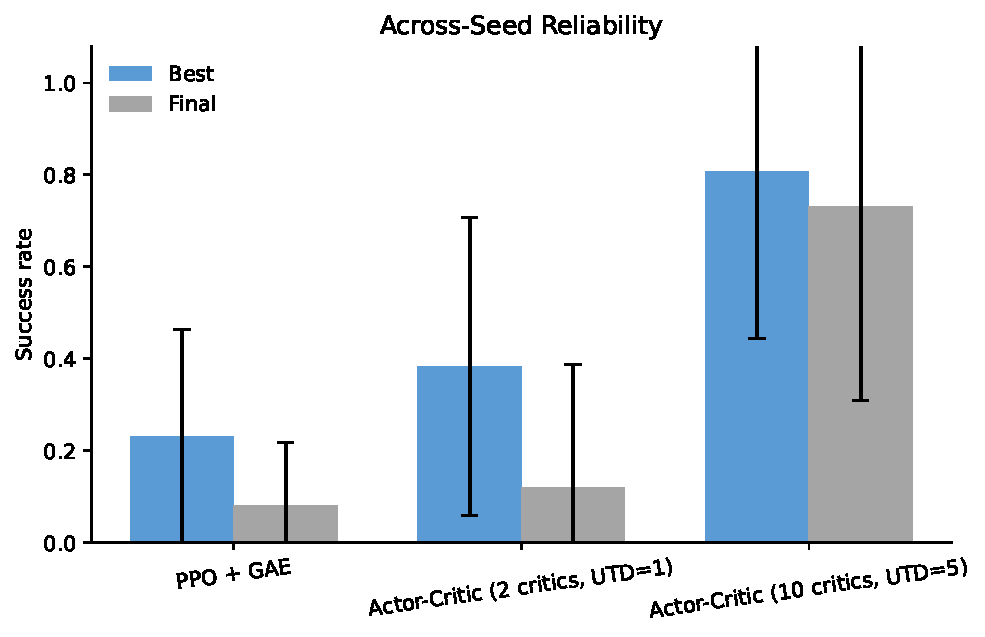
\includegraphics[width=\columnwidth]{success_distribution}
\caption{Best checkpoint 与 final checkpoint 的 across-seed 差异。}
\end{figure}
选择 best checkpoint 需要独立 validation tasks/seeds；若在 test curve 上挑最高点，
会产生 multiple-comparison bias。课程验收关心“是否在 budget 内达到阈值”，可报告 first
crossing frame；部署稳定性则更关心 final 与 rolling mean。

\subsection{公平比较的三个 Budget}
\begin{enumerate}
  \item environment frames：衡量真实交互成本；
  \item gradient updates/FLOPs：衡量训练计算；
  \item wall time：包含 simulator、data loader、evaluation 和日志。
\end{enumerate}
on-policy 与 off-policy 算法只按 frames 比较是不完整但有意义的。论文应明确主要 claim
是 sample efficiency 还是 total compute。

\section{调试顺序：从手算到长任务}
\begin{enumerate}
  \item \textbf{Tabular sanity check：}小 MDP 手算一个 update，确认 terminal mask；
  \item \textbf{Tensor tests：}检查 shape、finite、detach、gradient 和 parameter change；
  \item \textbf{Overfit demonstration：}BC loss 与 action MSE 应下降；
  \item \textbf{Short smoke：}数千 frames 验证 env、replay、eval.csv 和 checkpoint；
  \item \textbf{Single-seed curve：}确认 success 非零，再启动 multi-seed；
  \item \textbf{Ablation：}一次只改 $\lambda$、UTD 或 critic count 等可解释变量。
\end{enumerate}

\textbf{critic loss 下降但 return 不升。}可能是 replay 只含失败、Q scale 错误、
extrapolation error 或 actor 没有获得有效 gradient。\textbf{PPO ratio 爆炸。}检查
old log-prob 是否在 rollout 时保存，action dimensions 是否 sum，是否在 update 前改变
actor。\textbf{success 突然归零。}检查 actor std、Q overestimation、target lag、BC
regularization 和 evaluation action 是否使用 mean。

\section{系统设计题：机器人 Online RL 平台}
回答可分五层。\textbf{数据层：}replay 按 episode 分片，记录 policy version、task、
success、sensor calibration 与 intervention；demonstrations 单独 version。
\textbf{训练层：}actor 与 learner 解耦，prioritized sampling 要记录 correction，
checkpoint 包含 optimizer、target networks、normalizer 与 replay cursor。
\textbf{评价层：}固定 scenario bank，simulation 与 real-robot 分级，使用 confidence
interval 和 safety violations。\textbf{部署层：}动作 bounds、watchdog、latency
budget、fallback controller 和 human override。\textbf{监控层：}state/action drift、
critic disagreement、episode success、constraint cost 与 intervention rate。

真实机器人不应直接部署随机 exploration。可先在 simulation pretrain，以 demonstrations
初始化，再用 conservative action noise、safety shield 或 residual policy 逐步上线。
sim-to-real 的核心不是只随机化视觉，而是覆盖 dynamics、delay、contact、calibration 与
observation noise。

\section{高频面试问答}
\textbf{Q1：Q-learning 为什么会 overestimate？}max 选择与评估使用同一组带噪估计，
selection bias 使最大值偏高。Double-Q 解耦选择与评估，clipped double-Q 用 minimum
换取 conservative bias。

\textbf{Q2：PPO 是严格 on-policy 吗？}rollout 来自 frozen old policy；同一 rollout
多 epoch 后当前 policy 已变化，因此严格说产生轻微 off-policy。importance ratio 与
clip 控制偏离，但 replay buffer 长期复用不适合 PPO。

\textbf{Q3：GAE $\lambda$ 与 discount $\gamma$ 有何不同？}$\gamma$ 定义优化目标的
时间偏好；$\lambda$ 组合多步 estimators，主要调 bias--variance。实现中二者乘在一起，
语义不能混淆。

\textbf{Q4：为什么 actor 不直接用 replay action？}actor improvement 需要评估当前
policy action 的 $Q(s,\pi(s))$。replay action 用于 critic supervised target 或 BC；
若直接最大化 replay action likelihood，就退化为 behavior cloning。

\textbf{Q5：ensemble 和 double-Q 各解决什么？}double-Q 的 min 主要抑制
overestimation；ensemble 提供多个 error realizations、uncertainty proxy 和随机
subset。只有两个 critics 也可 double-Q，但不能充分估计 disagreement。

\textbf{Q6：何时提高 UTD？}interaction 贵、replay 足够多样、critic 稳定时。若 buffer
很小、policy 快速变化或 Q divergence，先降低 UTD、learning rate，增加 target lag 或
regularization。

\textbf{Q7：为什么 sparse reward 需要 demonstrations？}不是数学上必需，而是随机
exploration 的 hitting probability 太低。demonstrations 提供成功 state-action support，
让 critic 和 policy gradient 在有限 budget 内获得正信号。

\section{如何把本作业讲成项目经历}
使用“问题--证据--决策--结果”而非只说“实现 PPO”：
\begin{itemize}
  \item 问题：hammer binary reward 下 PPO 与 off-policy sample efficiency 差异；
  \item 证据：多 seed learning curves、first-crossing frames、GAE/UTD ablations；
  \item 决策：恢复官方 demonstrations，写 terminal/gradient tests，并行独立 jobs；
  \item 结果：PPO best \PPOBest，off-policy best \OffBaseBest，高 UTD best
  \OffUTDBest；
  \item 反思：frames、updates 和 wall time 是不同成本，best seed 不能代表可靠性。
\end{itemize}
这一表达同时展示理论推导、PyTorch、MuJoCo 环境、GPU 调度、统计方法和技术写作。

\section{面试前自检清单}
\begin{itemize}
  \item 能从 Bellman optimality 写出 terminal-aware Q update；
  \item 能从 log-derivative 推导 policy gradient 与 baseline 无偏性；
  \item 能手算 GAE recursion，并解释 $\lambda$ 两端；
  \item 能针对正负 advantage 分别解释 PPO clip；
  \item 能画出 actor、critic、target、replay 的 data flow；
  \item 能解释 double-Q、ensemble、target network 与 UTD 的不同作用；
  \item 能设计 multi-seed、frame/compute/wall-time 三预算实验；
  \item 能诊断 Q divergence、policy collapse 和 sparse reward；
  \item 能给机器人 online exploration 加入 safety boundary。
\end{itemize}

\section{结语}
Online RL 的难点不在单个 loss，而在多个近似同时耦合：policy 改变 data distribution，
critic bootstrap 自己生成 target，replay 引入 policy lag，有限 evaluation 又带来选择
bias。高质量候选人应能把每个稳定化组件对应到具体 failure mode，并用可复现 ablation
而不是单条最好曲线支持结论。

\bibliographystyle{plainnat}
\bibliography{../references}
\end{document}
